%
%
%
%
%
%
%


\chapter{Einführung in das Thema}           % Kapitelüberschrift, Ebene 1
\pagenumbering{arabic}                      % nur beim ersten Kapitel auswählen



%Abkürzungen verwenden: \ac{Name_Abkürzung} anstelle der Abkürzung einsetzen
% -> Beim ersten Kapitel werden
%


This will be an empty chapter
Vor Jahren waren \ac{KDE} die größten Vermittler der Welt. 
\\ % einzeiliger Zeilenumbruch (vgl. Str. + Enter

Des lässt sich auch an xx feststellen. Der Mehrwert Bla Bla \blindtext

\par % Zweizeiliger Zeilenumbruch ( Vgl. Enter)
\blindtext{}
\section{Unterkapitel}
\blindtext{}
\section{Noch eins}

\chapter{Grundlagen der Sterilisation}
\blindtext[1] \par
%Bild einfügen, Bildbezug im Text über ~\ref{fig:render} 

\begin{figure}[htb]
    \centering  
    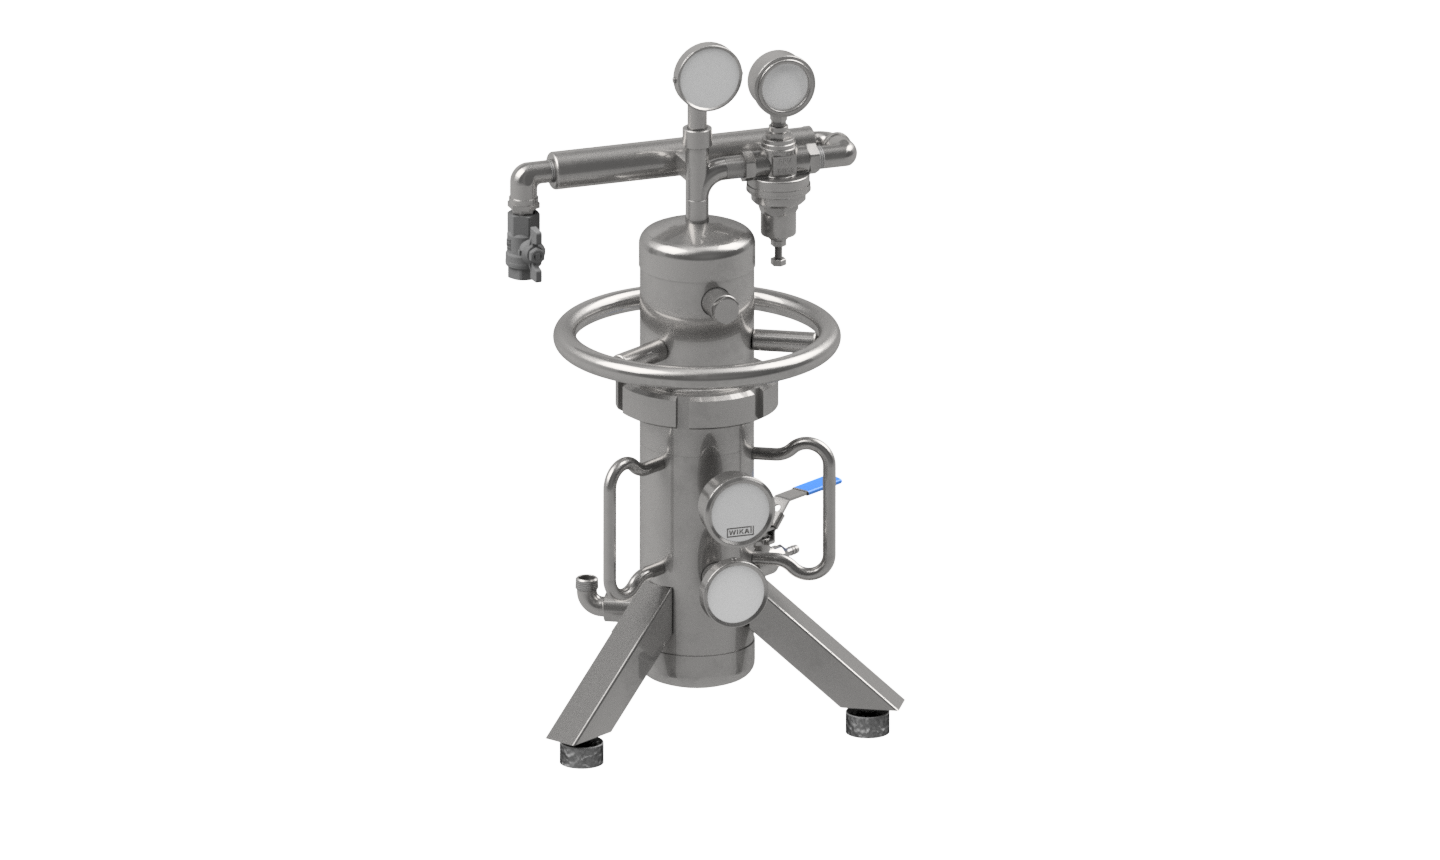
\includegraphics[keepaspectratio,width=\textwidth]{render.png}
    \caption{3D Darstellung des Dampfdruckbehälters}\label{fig:render}
\end{figure}

\par

Dies ist auch in Abbildung~\ref{fig:render} sehr gut zu erkennen (vgl. Abb.\ref{fig:render}).


\blindtext[2] \par


\section{Wahl der Dichtmittel}
\blindtext[2] \par

\section{Einflussgrößen auf die Auslegung nach AD2000}
\blindtext[1]


%Tabelle einfügen: 

\begin{table}[htb]
\centering
\begin{tabular}{|c|cc|} 
 \hline
 Einheit & Benennung & Kategorie \\ %[0.5ex] 
 \hline
 m & 6 & 8783 \\ 
 s & 7 & 78 \\
 V & 545 & 778\\
 A & 545 & 18744\\
 \hline
\end{tabular}
\caption{Eine sehr vielaussagende Tabelle}\label{vielaussagend}
\end{table}


Wie in Tabelle \ref{vielaussagend} zu erkennen, handelt es sich um eine sehr unwichtige Information, die hier gelistet ist.\blindtext[1]


\newpage
\chapter{Kapitel mit einigen Formeln}
\blindtext{}


%Aufschreiben von Formeln:
%1. Möglichkeit: Equatation - Umfeld


\begin{equation}
   a=b
    \label{eq:Eq3}          %Label Referenz für Textverweise
\end{equation}


%2. Möglichkeit: align Umgebung
%-> Vorteil: Intertext, Formatierung etc.

\begin{align}
\intertext{Zum einen gilt:} 
a+b&=c
\intertext{Zum anderen jedoch auch} 
b=c
\end{align}


Also was ist folglich c?



\blindtext{}

\begin{equation}\label{eq:Eq7}
a=b
\end{equation}



\begin{equation*}\label{eq:Eq2}         % Formel ohne Referenzzahl
   b=c
\end{equation*}

\begin{equation}
    \label{eq:Eq10}
    Y=Kd \ast \left(Xd + \frac{1}{Tn} + \int Xd\ dt + d\ \frac{Xd}{dt}\right)
\end{equation}


\newpage
\chapter{Kapitel mit Symbolen}

Hier stehen gleich einige Symbole, die im Symbolverzeichnis aufgelistet werden sollen. Zu finden sind die Quellen auch im Literaturverzeichnis unter~\cite[S.~49]{Wittel.2021b}
\[\symE=\symm \symc^2\]~\cite{VerbandderTUVe.V..2020}.

where \symE~is the energy \ldots


\newpage
\chapter{Fazit und sicherheitstechnische Beurteilung der Facharbeit}
\blindtext{}
\par
\blindtext{}
